\chapter{Writing Modules}
\section{Introduction}

The following chapter presents the \hrefinternal{http:///wiki/\#Modules_Interfaces}{modules interfaces} and explains \hrefinternal{http:///wiki/\#Writing_Custom_Modules}{how to write custom modules} for ASK.

\section{Module Interfaces}

Each kind of module has a strictly defined interface. For instance, every source module expects one configuration, one input and one output file.
This design makes possible to use as a source module any module implementation adhering to its interface. 
This section describes the interface for each kind of module.

Except if noted otherwise, each time a file is used in the modules below the format must be in ASK's \hrefinternal{http:///wiki/Application\_Characterization:_ASK:_Chapter_3:_Experiment_Setup\#Data_Exchange_Format}{data exchange format}.

\subsection{Bootstrap Interface}

A Bootstrap module selects the initial batch of points measured by ASK.

\emph{Interface:} \texttt{bootstrap \textless{}configuration\textgreater{} \textless{}output\_file\textgreater{}} 

\emph{Input:}
\begin{itemize}
	\item \texttt{configuration}: ASK configuration file
\end{itemize}

\emph{Output:}
\begin{itemize}
	\item \texttt{output\_file}: path of the output file. The output file contains a list of requested factors to be measured; therefore, it has no response column.
\end{itemize}

\subsection{Source Interface}

A source module computes the actual measures for the requested factors and returns the response.

\emph{Interface:} \texttt{source \textless{}configuration\textgreater{} \textless{}requested\_file\textgreater{} \textless{}output\_file\textgreater{}} 

\emph{Input:}
\begin{itemize}
	\item \texttt{configuration}: ASK configuration file
	\item \texttt{requested\_file}: path of the requested file containing the factors, which need to be measured
\end{itemize}

\emph{Output:}
\begin{itemize}
	\item \texttt{output\_file}: path of the output file. The output must include the factors passed on the requested file with an additional column containing the measured response for each factor combination.
\end{itemize}

\subsection{Model Interface}

A Model module builds a surrogate model for the experiment on the sampled points. It builds a function that predicts the response for every factor combination. The model predicts the unknown points, that is to say, the not measured ones.
Model modules are special, in that their output is module dependent. For instance, the GBM model produces General Boosted Models, the TGP model produces Tree Gaussian Process models. All the model modules distributed within ASK come in two parts:

\begin{itemize}
	\item model\_build, which allows to build the model
	\item model\_predict, which allows to use the model to predict unknown points
\end{itemize}

\emph{Interface:} \texttt{model\_build \textless{}configuration\textgreater{} \textless{}labelled\_file\textgreater{} \textless{}output\_file\textgreater{}} 

\emph{Input:}
\begin{itemize}
	\item \texttt{configuration}: ASK configuration file
	\item \texttt{labelled\_file}: path of the labelled file containing a list of measured points. It therefore contains factors columns and a response column.
\end{itemize}

\emph{Output:}
\begin{itemize}
	\item \texttt{output\_file}: path of the output file. The output file format depends on the module, it may be or may not be in ASK's \hrefinternal{http:///wiki/Application\_Characterization:_ASK:_Chapter_3:_Experiment_Setup\#Data_Exchange_Format}{data exchange format}. The output file contains the built model.
\end{itemize}

\emph{Interface:} \texttt{model\_predict \textless{}configuration.conf\textgreater{} \textless{}model\textgreater{} \textless{}requested\_file\textgreater{} \textless{}output\_file\textgreater{}} 

\emph{Input:}
\begin{itemize}
	\item \texttt{configuration}: ASK configuration file
	\item \texttt{model\_file}: path of the model file, produced by the associated \texttt{model\_build} command
	\item \texttt{requested\_file}: path of the labelled file containing a list of points to predict, therefore the response column is missing
\end{itemize}

\emph{Output:}
\begin{itemize}
	\item \texttt{output\_file}: path of the output file. The output file contains the same points passed in the requested\_file with a response column filled with the model's predictions.
\end{itemize}

\subsection{Sampler Interface}

A Sampler module selects a new batch of points to measure for every iteration after the first.
Bootstrap modules are in charge of selecting the first iteration's batch of points.

\emph{Interface:} \texttt{sampler \textless{}configuration\textgreater{} \textless{}input\_file\textgreater{} \textless{}output\_file\textgreater{}} 

\emph{Input:}
\begin{itemize}
	\item \texttt{configuration}: ASK configuration file
	\item \texttt{input\_file}: path of the input file containing the points that have already been measured an a column with their responses
\end{itemize}

\emph{Output:}
\begin{itemize}
	\item \texttt{output\_file}: path of the output file containing the new list of points to measure; therefore, it has no response column
\end{itemize}

\subsection{Control Interface}

A Control module decides when the sampling process ends. Two basic strategies are included in ASK: stopping when a predefined amount of points has been sampled or stopping when the accuracy improvement stays under a given threshold for a number of iterations.

\emph{Interface:} \texttt{points \textless{}configuration\textgreater{} \textless{}labelled\_file\textgreater{} \textless{}model\_file\textgreater{}} 

\emph{Input:}
\begin{itemize}
	\item \texttt{configuration}: ASK configuration file
	\item \texttt{labelled\_file}: path of the labelled file. It contains the points that have already been measured, it has a response column
	\item \texttt{model\_file}: path of the model file generated by the model module
\end{itemize}

\emph{Output:}
\begin{itemize}
	\item Control modules should return exit code 254 to stop the experiment, or any other code to pursue the experiment.
\end{itemize}

\subsection{Reporter Interface}

A Reporter module produces detailed statistics about the sampling.

\emph{Interface:} \texttt{reporter \textless{}configuration\textgreater{} \textless{}iteration\textgreater{} \textless{}labelled\_file\textgreater{} \textless{}newly\_labelled\_file\textgreater{} \textless{}model\_file\textgreater{}} 

\emph{Input:}
\begin{itemize}
	\item \texttt{configuration}: ASK configuration file
	\item \texttt{iteration}: iteration number, the bootstrap iteration is numbered 0
	\item \texttt{labelled\_file}: path of the labelled file containing the points that have already been measured, it has a response column
	\item \texttt{newly\_labelled\_file}: path of the newly labelled file containing the points that have been measured in the last iteration, it has a response column
	\item \texttt{model\_file}: path of the model file generated by the model module
\end{itemize}

\emph{Output:}
\begin{itemize}
	\item None required.
\end{itemize}

\section{Writing Custom Modules}

Custom modules may be written in any chosen language as long as they adhere to the \hrefinternal{http:///wiki/\#Module_interfaces}{module interfaces}.
As an example, the following section shows how to design a simple bootstrap module baptized Grid.

The grid module selects points regularly distributed in a grid. To make things simpler, it will only work with integer factors. The module is written in Python.

The grid module takes one parameter, \texttt{grid\_size}, which is the grid size. 
Supposing the design space has two factors x and y varying between 0 and 10, a grid size of 2 will select points (0,0), (0,2), (0,4) ... (0,10), (2,0), (2,2) ... (10,10).

\subsection{Input Parser}

The first step is writing a parser adhering to the \hrefinternal{http:///wiki/\#Bootstrap_Interface}{bootstrap interface}:
\begin{minted}{bash}
bootstrap <configuration> <output_file>
\end{minted}

In the example, the argparse module will be used:

\begin{minted}{python}
#!/usr/bin/env python
if __name__ == "__main__":
  import argparse
  parser = argparse.ArgumentParser(description="Sample the design space in a" 
             " grid fashion")
  parser.add_argument("configuration")
  parser.add_argument("output_file")
  args = parser.parse_args()
\end{minted}

After parsing the command line arguments, the module needs to parse the configuration file. ASK already provides a library for this purpose in python and in R.

\begin{minted}{python}
from common.configuration import Configuration
conf = Configuration(args.configuration)
\end{minted}

The conf object can be used to retrieve configurations values. To retrieve the \texttt{grid\_size} parameter, one can use:
\begin{minted}{python}
grid_size = conf("modules.bootstrap.params.grid_size")
\end{minted}

In the above code, if the parameter is missing, or is of the wrong type, the module fails and an error is logged. Fortunately, the conf object handles type checking and default values substituting the above code with:

\begin{minted}{python}
grid_size = conf("modules.bootstrap.params.grid_size", int, 1)
\end{minted}

Now, if the parameter is of the wrong type, an appropriate message is raised. Moreover, if the \texttt{grid\_size} parameter is missing, the default 1 value is used. 

Then the module retrieves the factors's configuration and checks that only integer factors were used:

\begin{minted}{python}
from common.util import fatal
factors = conf("factors")
for f in factors:
   if f["type"] != "integer":
     fatal("Grid bootstrap only works with integer factors.")
\end{minted}

Finally, pass all the input information to an appropriate function:
\begin{minted}{python}
grid_bootstrap(args.output_file, grid_size, factors)
\end{minted}

\subsection{Bootstrap Logic}

The previous code ensures that all the arguments are correctly parsed and strictly adheres to the \hrefinternal{http:///wiki/\#Bootstrap_Interface}{bootstrap interface}.
All that remains is writing the logic of the module. First, for each factor, the list of values in the grid is computed.

\begin{minted}{python}
def grid_bootstrap(output, grid_size, factors):
  from itertools import product
  coords = []
  for f in factors:
      coords.append(xrange(f["range"]["min"], f["range"]["max"] + 1, grid_size))
\end{minted}

Then, the module computes a Cartesian product of the previous values and writes the coordinates in \hrefinternal{http:///wiki/Application\_Characterization:_ASK:_Chapter_3:_Experiment_Setup\#Data_Exchange_Format}{ASK's data exchange format}:

\begin{minted}{python}
  out = file(output, "w")
  for c in product(*coords):
      out.write(" ".join(map(str,c)) + "\n")
  out.close()
\end{minted}

The custom module is now complete. It can be used as a drop-in replacement for an existing bootstrap module.
For example, changing the bootstrap module to ``grid'' inside \texttt{examples/face/experiment.conf} with a grid\_size of 20, produces the following report:

\begin{center}
  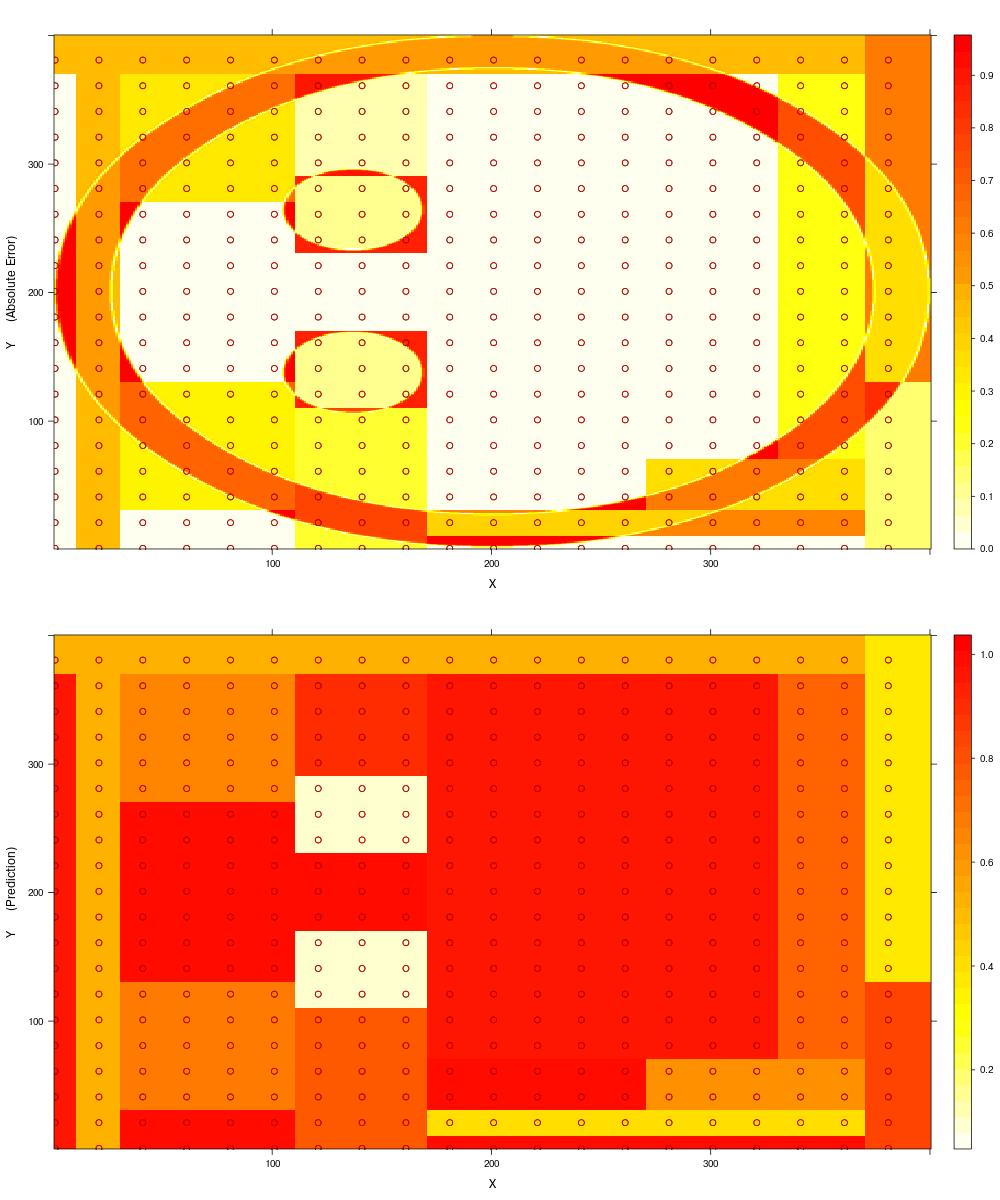
\includegraphics[width=\textwidth]{figures/ASK-Custom-Grid.png}
\end{center}


